\documentclass[
11pt, % The default document font size, options: 10pt, 11pt, 12pt
%codirector, % Uncomment to add a codirector to the title page
]{charter} 




% El títulos de la memoria, se usa en la carátula y se puede usar el cualquier lugar del documento con el comando \ttitle
\titulo{Sistema de gestión y monitoreo de CO$_{2}$ para la vigilancia de la salud de los trabajadores con riesgo de exposición al COVID-19 u otras enfermedades respiratorias   } 

% Nombre del posgrado, se usa en la carátula y se puede usar el cualquier lugar del documento con el comando \degreename
%\posgrado{Carrera de Especialización en Sistemas Embebidos} 
\posgrado{Carrera de Especialización en Internet de las Cosas} 
%\posgrado{Carrera de Especialización en Intelegencia Artificial}
%\posgrado{Maestría en Sistemas Embebidos} 
%\posgrado{Maestría en Internet de las cosas}

% Tu nombre, se puede usar el cualquier lugar del documento con el comando \authorname
\autor{Ing. Jhonatan Alexander Juño Garcia} 

% El nombre del director y co-director, se puede usar el cualquier lugar del documento con el comando \supname y \cosupname y \pertesupname y \pertecosupname
\director{Esp. Ing. Claudio Omar Biale}
\pertenenciaDirector{FIUBA} 
% FIXME:NO IMPLEMENTADO EL CODIRECTOR ni su pertenencia
\codirector{John Doe} % para que aparezca en la portada se debe descomentar la opción codirector en el documentclass
\pertenenciaCoDirector{FIUBA}

% Nombre del cliente, quien va a aprobar los resultados del proyecto, se puede usar con el comando \clientename y \empclientename
\cliente{Manuel Behar}
\empresaCliente{Loratech S.A.C.}

% Nombre y pertenencia de los jurados, se pueden usar el cualquier lugar del documento con el comando \jurunoname, \jurdosname y \jurtresname y \perteunoname, \pertedosname y \pertetresname.
\juradoUno{Nombre y Apellido (1)}
\pertenenciaJurUno{pertenencia (1)} 
\juradoDos{Nombre y Apellido (2)}
\pertenenciaJurDos{pertenencia (2)}
\juradoTres{Nombre y Apellido (3)}
\pertenenciaJurTres{pertenencia (3)}
 
\fechaINICIO{25 de abril de 2023}		%Fecha de inicio de la cursada de GdP \fechaInicioName
\fechaFINALPlan{13 de junio de 2023} 	%Fecha de final de cursada de GdP
\fechaFINALTrabajo{en el mes de diciembre de 2023}	%Fecha de defensa pública del trabajo final


\begin{document}

\maketitle
\thispagestyle{empty}
\pagebreak


\thispagestyle{empty}
{\setlength{\parskip}{0pt}
\tableofcontents{}
}
\pagebreak


\section*{Registros de cambios}
\label{sec:registro}


\begin{table}[ht]
\label{tab:registro}
\centering
\begin{tabularx}{\linewidth}{@{}|c|X|c|@{}}
\hline
\rowcolor[HTML]{C0C0C0} 
Revisión & \multicolumn{1}{c|}{\cellcolor[HTML]{C0C0C0}Detalles de los cambios realizados} & Fecha      \\ \hline
0      & Creación del documento                                 &\fechaInicioName \\ \hline
1      & Se completa hasta el punto 5 inclusive                 & 9 de mayo de 2023 \\ \hline
2      & Se corrige la primera entrega y se completa hasta el punto 9 inclusive & 16 de mayo de 2023\\ \hline
3	   & Se corrige la segunda entrega y se completa hasta el punto 12 inclusive & 24 de mayo de 2023\\ \hline
4	   & Se corrige la tercera entrega y se completa la planificación & 1 de junio de 2023\\ \hline
%		  Así                                                    & dd/mm/aaaa \\ \hline
%3      & Se completa hasta el punto 11 inclusive                & dd/mm/aaaa \\ \hline
%4      & Se completa el plan	                                 & dd/mm/aaaa \\ \hline
\end{tabularx}
\end{table}

\pagebreak



\section*{Acta de constitución del proyecto}
\label{sec:acta}

\begin{flushright}
Buenos Aires, \fechaInicioName
\end{flushright}

\vspace{2cm}

Por medio de la presente se acuerda con el \authorname\hspace{1px} que su Trabajo Final de la \degreename\hspace{1px} se titulará ``\ttitle''. El trabajo consistirá esencialmente en el desarrollo de un sistema de gestión y monitoreo para  medidores inalámbricos de dióxido de carbono (CO$_{2}$), que permitirá registrar los niveles de CO$_{2}$ en tiempo real en los ambientes de trabajo. Esto es parte de una estrategia del gobierno de la República del Perú para un retorno seguro a las labores presenciales en los centros de trabajo. Este trabajo tendrá un presupuesto preliminar estimado de 660 h de trabajo y S/75140,00 PEN (\$20308,11 USD), con fecha de inicio el \fechaInicioName\hspace{1px} y fecha de presentación pública \fechaFinalName.

Se adjunta a esta acta la planificación inicial.

\vfill

% Esta parte se construye sola con la información que hayan cargado en el preámbulo del documento y no debe modificarla
\begin{table}[ht]
\centering
\begin{tabular}{ccc}
\begin{tabular}[c]{@{}c@{}}Dr. Ing. Ariel Lutenberg \\ Director posgrado FIUBA\end{tabular} & \hspace{2cm} & \begin{tabular}[c]{@{}c@{}}\clientename \\ \empclientename \end{tabular} \vspace{2.5cm} \\ 
\multicolumn{3}{c}{\begin{tabular}[c]{@{}c@{}} \supname \\ Director del Trabajo Final\end{tabular}} \vspace{2.5cm} \\
%\begin{tabular}[c]{@{}c@{}}\jurunoname \\ Jurado del Trabajo Final\end{tabular}     &  & \begin{tabular}[c]{@{}c@{}}\jurdosname\\ Jurado del Trabajo Final\end{tabular}  \vspace{2.5cm}  \\
%\multicolumn{3}{c}{\begin{tabular}[c]{@{}c@{}} \jurtresname\\ Jurado del Trabajo Final\end{tabular}} \vspace{.5cm}                                                                     
\end{tabular}
\end{table}




\section{1. Descripción técnica-conceptual del proyecto a realizar}
\label{sec:descripcion}

El presente trabajo surge a partir de un requerimiento de la empresa donde trabaja el responsable y que esta ha notado la problemática a la que se enfrentan muchas empresas en la transición del trabajo remoto a la presencialidad después de la pandemia por el coronavirus SARS-CoV-2 (COVID-19) en la República del Perú. El Ministerio de Salud y el Ministerio del Trabajo han dispuesto nuevas normativas de seguridad y salud en el trabajo que las empresas deben cumplir para garantizar un retorno seguro a las labores presenciales. Dentro de este contexto, una de las normas más importantes se refiere a los ambientes de trabajo saludables, en particular a la calidad del aire y la correcta ventilación de los espacios laborales. 

Dentro de los parámetros que determinan la calidad de aire en un centro de trabajo el CO$_{2}$ es uno de los más importantes, ya que está directamente relacionado con la actividad de los trabajadores y la exhalación generada durante la jornada laboral. Niveles altos de CO$_{2}$ en el aire pueden ser causados por la alta aglomeración de personas o una deficiente ventilación del lugar. Esto último genera el ambiente propicio para el incremento del riesgo de exposición a enfermedades respiratorias como SARS-CoV-2 (COVID-19), la influenza, gripe, entre otras.

Hasta el momento, las evaluaciones de la calidad del aire en ambientes de trabajo se han basado en mediciones puntuales del CO$_{2}$ realizadas con equipos manuales. Estas mediciones se llevaban a cabo generalmente una o dos veces al año, incluso con periodos más prolongados. Sin embargo, este enfoque no permite un seguimiento continuo de los niveles de CO$_{2}$, ya que solo muestran información de un momento específico.

A raíz del COVID-19 y sus efectos, a través de varios decretos del Ministerio de Salud y el Ministerio de Trabajo, se han dispuesto una serie de directivas para la medición de calidad de aire en ambientes de trabajo, específicamente mediante la medición del CO$_{2}$. La norma establece alcances sobre el uso de equipos de medición de CO$_{2}$ como parte de los planes de acción para mantener espacios de trabajo ventilados, limpios y seguros.

De lo expuesto, surge la necesidad de desarrollar un sistema de gestión y monitoreo de CO$_{2}$. Este sistema debe gestionar los equipos de medición y monitorizar los valores medidos para el control de la calidad de aire en los ambientes de trabajo. Además contará con alarmas programadas y visualización en tiempo real de niveles de CO$_{2}$. Esto permitirá la implementación de mejoras en los ambientes de trabajo, como protocolos para la apertura de ventanas, la adecuación de aforos, mejor ventilación y/o instalación de sistemas de ventilación forzada entre otros, lo que reducirá el riesgo de exposición a enfermedades respiratorias y mejorará las condiciones de trabajo a largo plazo.

El proyecto se dividirá en dos etapas para alcanzar los objetivos. La primera etapa consistirá en la implementación de una red de comunicación para los equipos de medición de CO$_{2}$. Esta red se utilizará para las pruebas y servirá para elaborar el procedimiento de configuración e instalación de equipos que se utilizará cuando se lleve la solución a un cliente. La segunda etapa se enfocará en el desarrollo del sistema de gestión y de monitoreo.

En la Figura \ref{fig:diagBloque1} se muestra el diagrama en bloques de la red de comunicación, que se compone de los siguientes elementos:

\begin{itemize}
	\item Equipos de medición de CO$_{2}$ con comunicación LoRaWAN.
	\item \textit{Gateway} de comunicación LoRaWAN.
	\item \textit{Network server}.
	\item Sistema de gestión y monitoreo - \textit{application server}.
\end{itemize}

\begin{figure}[htpb]
\centering 
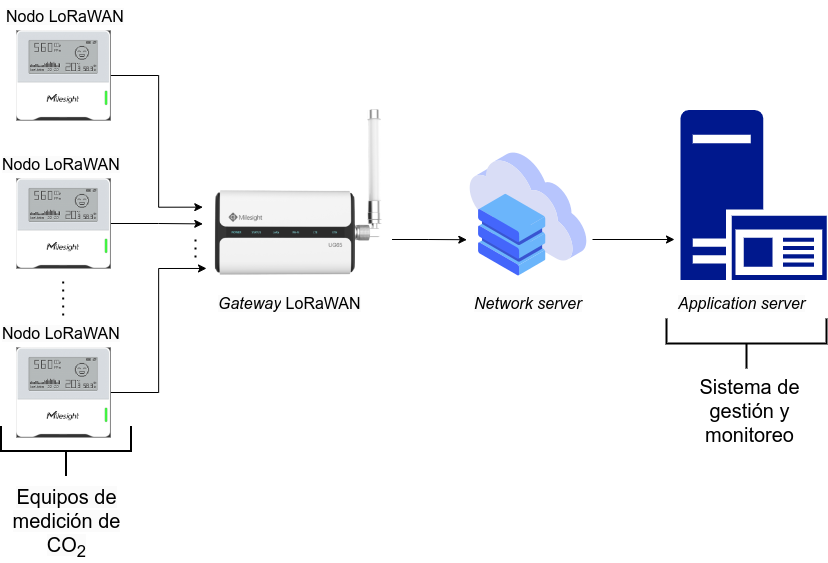
\includegraphics[width=.9\textwidth]{./Figuras/diagBloque1.png}
\caption{Diagrama de bloques de la red de comunicación.}
\label{fig:diagBloque1}
\end{figure}
\vspace{25px}

El objetivo de la red de comunicación es llevar los valores medidos de CO$_{2}$ al sistema de gestión y monitoreo. La comunicación que usará el equipo de medición y \textit{gateway} será LoRa con protocolo LoRaWAN. El \textit{network server }permitirá la conexión con el sistema de gestión y monitoreo.

En la Figura \ref{fig:diagBloque2} se muestra el diagrama del sistema de gestión y monitoreo de medidores de CO$_{2}$ donde se observan los siguientes elementos:
\begin{itemize}
	\item \textit{Network server}.
	\item Análisis en Node.JS.
	\item Plataforma de \textit{edge computing}.
	\item Base de datos.
	\item Aplicación de visualización.
\end{itemize}

Esta parte del proyecto es crítica y demandará un esfuerzo significativo en el desarrollo. Será necesario prestar especial atención para cumplir con todos los requerimientos que se planteen en esta planificación.

\begin{figure}[htpb]
\centering 
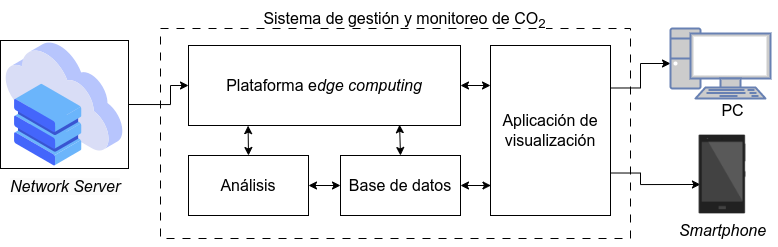
\includegraphics[width=\textwidth]{./Figuras/diagBloque2.png}
\caption{Diagrama en bloques del sistema de gestión de medidores de CO$_{2}$}.
\label{fig:diagBloque2}
\end{figure}
\vspace{25px}



\section{2. Identificación y análisis de los interesados}
\label{sec:interesados}
En la siguiente tabla se muestra de forma resumida los \textit{stakeholders} del presente proyecto.
\begin{table}[ht]
\begin{tabularx}{\linewidth}{@{}|l|X|X|l|@{}}
\hline
\rowcolor[HTML]{C0C0C0} 
Rol           & Nombre y Apellido & Organización 	& Puesto 	\\ \hline
Auspiciante   & Guillermo Amaro   &\empclientename  & Director-Gerente       	\\ \hline
Cliente       & \clientename      &\empclientename	& Gerente General\\ \hline
Responsable   & \authorname       & FIUBA        	& Alumno 	\\ \hline
Orientador    & \supname	      & \pertesupname 	& Director Trabajo Final \\ \hline
Usuario final & Clientes de \empclientename		    &-       & -   	\\ \hline
\end{tabularx}
\end{table}

Principales características de cada interesado.
\begin{itemize}
	\item Auspiciante: Guillermo Amaro, asignará los recursos e instalaciones de la empresa para la elaboración del proyecto. Es riguroso y exigente con la rendición de gastos.
	\item Cliente: \clientename, participará activamente, con comentarios y sugerencias durante el desarrollo así como en la revisión de entregables.
	\item Responsable: \authorname.
	\item Usuario final: los usuarios finales serán las empresas a las que se les brindará el sistema de gestión y monitoreo de CO$_{2}$ (centros de oficinas, bancos, colegios y universidades, hospitales y clínicas, tiendas por departamentos, centros comerciales, etc).
\end{itemize}

\section{3. Propósito del proyecto}
\label{sec:proposito}
El propósito de este proyecto es desarrollar un sistema de gestión y monitoreo para los equipos de medición de CO$_{2}$ en ambientes laborales. Este sistema será utilizado por las empresas para gestionar ambientes de trabajo saludables y tomar acciones de control para reducir el riesgo de exposición al COVID-19 y otras enfermedades respiratorias. Esto se hace en respuesta a la nueva demanda que están teniendo las empresas debido a las nuevas disposiciones en materia de seguridad y salud en el trabajo promovidas por el Ministerio de Salud y el Ministerio del Trabajo en la República del Perú.

\section{4. Alcance del proyecto}
\label{sec:alcance}
El alcance de este proyecto está orientado a desarrollar la red de comunicación y el sistema de software. Los siguientes puntos serán tomados en cuenta para el desarrollo del proyecto:
\begin{itemize}
	\item Dimensionamiento de la red de comunicación LoRaWAN.
	\item Configuración de equipos (medidor de CO$_{2}$, \textit{gateway} LoRaWAN) y \textit{network server}. 
	\item Elaboración de documentación detallada del dimensionamiento de la red LoRaWAN, configuración de equipos y \textit{network server}.
	\item Desarrollo del \textit{Backend}, donde se implementará la aplicación de \textit{edge computing} y la base de datos.
	\item Desarrollo del \textit{frontend}, basado en una aplicación web desde donde los usuarios accederán a la información generada.
	\item Toda la solución correrá de forma local en un ordenador que actuará de servidor.
\end{itemize}

El presente proyecto no incluye los siguientes puntos que serán analizados para una futura implementación:
\begin{itemize}
	\item Montar la solución en un servicio \textit{cloud}.
	\item Desarrollo de una aplicación móvil nativa para el acceso al sistema.
	\item Análisis mas exhaustivo de los datos para aprendizaje automático.
\end{itemize}
	

\section{5. Supuestos del proyecto}
\label{sec:supuestos}
Para el desarrollo del presente proyecto se supone que:

\begin{itemize}
	\item Los equipos LoRaWAN cuentan con la homologación y permiso correspondiente del Ministerio de Transportes y Comunicaciones para ser utilizados en la República del Perú.
	\item Todos los equipos necesarios para el proyecto han sido adquiridos y se dispone de varias unidades para llevar a cabo las pruebas correspondientes.
	\item Se dispone de un ordenador de escritorio que será utilizado como servidor, el cual ha sido preparado para su configuración.
	\item Los permisos necesarios para la instalación de los equipos en el cliente de prueba han sido obtenidos. 
	\item Se ha asignado un ambiente dedicado en el laboratorio de la empresa para el desarrollo del proyecto.
	\item La empresa ha garantizado el tiempo necesario y apoyo para la obtención de recursos adicionales que puedan ser necesarios durante el proyecto.
\end{itemize}

\section{6. Requerimientos}
\label{sec:requerimientos}
Los requerimientos del proyecto fueron establecidos en una reunión en la que participaron todos los \textit{stakeholders}. Todos los requerimientos están alineados con las nuevas disposiciones establecidas por el Ministerio de Salud y el Ministerio de Trabajo de la República del Perú, tal como se resumen en la Directiva Administrativa N° 339 - MINSA/DGIESP - 2023. Dicho documento establece los requerimientos mínimos para el sistema de medición de CO$_{2}$. A continuación se detallan los requerimientos que se tendrán en cuenta para el proyecto.

\begin{enumerate}
	\item Requerimientos de la red de comunicación y los equipos.
		\begin{enumerate}
			\item El protocolo de comunicación para los equipos de medición de CO$_{2}$ y el \textit{gateway} deberá ser LoRaWAN. El fabricante de dichos equipos debe estar certificado por la LoRa Alliance.
			\item Los equipos deberán operar en la banda de frecuencias autorizada para LoRaWAN en la República del Perú, que abarca desde 915 MHz hasta 928 MHz. 
			 \item La red de comunicación deberá tener la capacidad de brindar cobertura total en los ambientes laborales. Se establece como requisito que los valores de RSSI (indicador de la fuerza de la señal recibida) en los equipos de medición sean superiores a -120 dBm.
			\item El \textit{gateway} deberá contar con un \textit{network server} embebido y admitir múltiples opciones de \textit{backhaul} como Ethernet, Wi-Fi y red celular.
			\item El \textit{gateway} deberá incluir una interfaz de configuración que permita realizar una integración con el sistema de gestión y monitoreo a través del protocolo HTTP.
			\item El equipo de medición de CO$_{2}$ deberá contar con una pantalla que muestre el valor medido. El rango de medición deberá estar comprendido entre 400 y 1500 ppm (partículas por millón).
			\item El equipo de medición de CO$_{2}$ deberá permitir la configuración remota de parámetros, como el período de transmisión y los umbrales mínimo y máximo para el envío de alertas.	
		\end{enumerate}
	\item Requerimientos del sistema de gestión y monitoreo de medidores de CO$_{2}$.
		\begin{enumerate}
			\item Se deberá implementar un servidor con sistema operativo Ubuntu Server versión 22.04 LTS o superior.
			\item La base de datos utilizada deberá ser del tipo relacional.
			\item Se deberá implementar una API-REST con  NodeJS.
			\item Los \textit{scripts} para análisis de datos se codificarán con NodeJS.
			\item Se deberá utilizar la aplicación de \textit{edge computing} TagoCore. 
			\item Se deberá diseñar una aplicación web con Angular. 
			\item La aplicación web deberá implementar varios \textit{dashboards} para  el \textit{login} de los usuarios, la visualización de los datos, gestión de alarmas y generar reportes con los valores medidos.
			\item La aplicación deberá generar alarmas en tiempo real y notificar al usuario en el momento. 
		\end{enumerate}
	\item Requerimientos de documentación.
		\begin{enumerate}
			\item Se documentará el procedimiento de configuración de equipos y el protocolo de instalación en el local del cliente).
			\item Se documentará el proceso de levantamiento del sistema de gestión y monitoreo de medidores sobre el servidor (requisitos de \textit{hardware} para el servidor, \textit{software} empleado y  procedimiento de instalación).
			\item Todo el código desarrollado será cargado al repositorio de GitHub de la compañía.
			\item Se elaborará un manual de uso del equipo de medición y la aplicación web para los usuarios finales.
		\end{enumerate}
	\item Requerimiento de \textit{testing}
		\begin{enumerate}
			\item Se deberá implementar una prueba inicial en las oficinas de la empresa para evaluar el funcionamiento.
			\item Se deberán simular valores anormales del CO$_{2}$, para verificar el comportamiento del sistema y la generación de alarmas.
			\end{enumerate}
\end{enumerate}

\section{7. Historias de usuarios (\textit{Product backlog})}
\label{sec:backlog}
Se identifican los siguientes roles:
\begin{itemize}
 \item Cliente: es quien que solicitó el proyecto.
 \item Usuario final: empresas a las que se les brindará el sistema de medición y monitoreo de CO$_{2}$. Dentro de las empresas existirá un usuario específico directo que será responsable del uso de los equipos y del sistema de medición. Para las historias vamos a considerar los siguientes usuarios específicos: 
 	\begin{itemize}
 	\item Jefe de salud ocupacional de un edificio empresarial.
 	\item Supervisor de seguridad en una industria.
 	\item Director de un colegio inicial.
 	\item Administrador de un banco.
 	\item Administrador de un centro comercial.
 	\end{itemize} 
 \end{itemize} 
 
Criterio para la asignación de \textit{story points} basada en la serie de Fibonacci:

\begin{center}
\begin{tabular}{|c|c|c|c|}
\hline 
Peso & Dificultad & Complejidad & Riesgo \\ 
\hline 
Bajo & 1 & 1 & 1 \\ 
\hline 
Medio & 3 & 5 & 5 \\ 
\hline 
Alto & 5 & 8 & 13 \\ 
\hline 
\end{tabular} 
\end{center}

A continuación se listan las historias de usuario:
\begin{enumerate}
	\item Como cliente, quiero un procedimiento de configuración e instalación de equipos claro y conciso para lograr una instalación rápida y sencilla en los locales de los usuarios finales.
	\begin{itemize}
 		\item Dificultad: 5
 		\item Complejidad: 5
	 	\item Riesgo: 1
	 	\item \textit{Story points}: 13
 	\end{itemize} 
	\item Como jefe de salud ocupacional de un edificio empresarial, quiero determinar las áreas con mayor aglomeración de personas dentro del edificio para generar mis planes de control.
	\begin{itemize}
 		\item Dificultad: 3
 		\item Complejidad: 5
	 	\item Riesgo: 5
	 	\item \textit{Story points}: 13
 	\end{itemize} 
	\item Como supervisor de seguridad en una industria, quiero monitorear los niveles de  CO$_{2}$ en distintos puntos para plantear mis estrategias de control ocupacional.
	\begin{itemize}
 		\item Dificultad: 3
 		\item Complejidad: 5
	 	\item Riesgo: 5
	 	\item \textit{Story points}: 13
 	\end{itemize} 
	\item Como director de un colegio inicial, quiero recibir notificaciones cuando se superen los límites establecidos para poder generar planes de prevención de contagios de enfermedades respiratorias entre los estudiantes.
	\begin{itemize}
 		\item Dificultad: 1
 		\item Complejidad: 5
	 	\item Riesgo: 13
	 	\item \textit{Story points}: 21
 	\end{itemize} 
 	\item Como administrador de un banco, quiero que la aplicación muestre la calidad del aire y que esta información pueda ser vista por los clientes para concientizar sobre el respeto a los aforos establecidos.
 	\begin{itemize}
 		\item Dificultad: 3
 		\item Complejidad: 5
	 	\item Riesgo: 5
	 	\item \textit{Story points}: 13
 	\end{itemize} 
 	\item Como administrador de un centro comercial, quiero poder ver los reportes mensuales de mediciones de CO$_{2}$ y el historial de alarmas para poder ajustar mis controles de aforo en las distintas áreas. 
 	\begin{itemize}
 		\item Dificultad: 3
 		\item Complejidad: 8
	 	\item Riesgo: 1
	 	\item \textit{Story points}: 13
 	\end{itemize} 
\end{enumerate}
\section{8. Entregables principales del proyecto}
\label{sec:entregables}

\begin{itemize}
	\item Manual de configuración e instalación de equipos. Incluye descripción de actividades y gráficos.
	\item Un servidor configurado, con la aplicación web corriendo y listo para su uso.
	\item Manual de configuración del servidor. Incluye todos los pasos y requisitos en caso de que se desee migrar el sistema y aplicación web a otro servidor.
	\item Manual de uso de la aplicación. Para entrega a los usuarios finales.
	\item Código fuente del sistema en el repositorio GitHub de la empresa.
	\item Informe final.
\end{itemize}

\section{9. Desglose del trabajo en tareas}
\label{sec:wbs}
\begin{enumerate}
\item Planificación y definición del proyecto. (40 h)
	\begin{enumerate}
	\item Análisis del mercado, normativas y soluciones similares. (10 h)
	\item Definición del alcance, requerimientos y tareas. (10 h)
	\item Elaboración del plan de proyecto. (20 h)
	\end{enumerate}
\item Dimensionamiento de la red de comunicación y configuración de equipos.  (30 h)
	\begin{enumerate}
	\item Configuración del \textit{gateway} (\textit{network server }embebido, bandas de frecuencias). (5 h)
	\item Configuración del equipo de medición de CO$_{2}$ (registro en el \textit{network server} y ajuste de las subbandas de frecuencias). (5 h)
	\item Primera prueba de conexión, verificación en los equipos de los niveles de RSSI. (5 h)
	\item Corrección de la ubicación del \textit{gateway} y los equipos con valores de RSSI inferiores al mínimo. Realización de nuevas mediciones y validación (5 h).
	\item Documentación del dimensionamiento de la red. (10 h)
	\end{enumerate}
\item Configuración del servidor.  (22 h)
	\begin{enumerate}
	\item Instalación de las aplicaciones requeridas. (5 h)
		\begin{enumerate}
		\item[3.1.1]Instalación del sistema operativo.	(2 h)
		\item[3.1.2]Instalación del la base de datos MySQL. (0,5 h)
		\item[3.1.3]Instalación del paquete de NodeJS.	(0,5 h)
		\item[3.1.4]Instalación de la aplicación TagoCore. (1 h)
		\item[3.1.5]Instalación de Visual Studio Code + \textit{plugins} requeridos. (1 h)
		\end{enumerate}
	\item  Configuración de TagoCore. (2 h)
		\begin{enumerate}
		\item[3.2.1]Ejecución de la aplicación. 	(0,5 h)
		\item[3.2.2]Integración con la base de datos. (1 h)
		\item[3.2.3]Configuración del path de ejecución de NodeJS sobre Tagocore. (0,5 h)
		\end{enumerate}
	\item Creación de las tablas de datos adicionales. (10 h)
		\begin{enumerate}
		\item[3.3.1]Definición de las tablas de datos adicionales no gestionadas por Tagocore. 	(6 h)
		\item[3.3.2]Creación de las tablas de datos adicionales. (4 h)
		\end{enumerate}
	\item Documentación de la configuración del servidor. (5 h)
	\end{enumerate}
\item Conexión del \textit{network server} a TagoCore. (20 h)
	\begin{enumerate}
	\item Registro de los medidores de CO$_{2}$ en TagoCore. (1 h)
	\item Obtención de los \textit{tokens} HTTP en TagoCore. (0,5 h)
	\item Registro de los \textit{tokens} en el \textit{network server}. (0,5 h)
	\item Prueba de conexión inicial. (3 h)
	\item \textit{Parseo} de datos recibidos en TagoCore. Validación de los datos obtenidos con los valores mostrados en el equipo. (5 h)
	\item Documentación de la conexión del \textit{network server} a TagoCore. (10 h)
	\end{enumerate}
\item Desarrollo de la API-REST - \textit{backend}.   (130 h)
	\begin{enumerate}
	\item Implementación de un CRUD (\textit{Create, Read, Update and Delete}) para la base de datos.	(30 h)	
	\item Implementación del método para envió de \textit{emails} y SMS. (15 h)
	\item Implementación del método para la gestión de equipos. (19 h)
	\item Implementación del método para la gestión de usuarios. (18 h)
	\item Implementación del método para la gestión de reglas y alarmas. (19 h)
	\item Implementación del método para la gestión de reportes. (19 h)
	\item Documentación del desarrollo de la API-REST. (10 h)
	\end{enumerate}

\item Desarrollo de la aplicación en Angular - \textit{frontend}.   (240 h)
	\begin{enumerate}
	\item Programación del \textit{login} de usuarios. (40 h) 
	\item Programación del \textit{dashboard} de ubicación y estado de los equipos. (40 h)
	\item Programación del \textit{dashboard} de visualización de los datos.  (40 h)
	\item Programación del \textit{dashboard} de configuración de reglas y alertas del sistema. (40 h)
	\item Programación del \textit{dashboard} para la generación de reportes. (40 h)
	\item Pruebas y test de la aplicación con datos simulados. (20 h)
	\item Pruebas y test de la aplicación con equipo de medición conectado. (10 h)
	\item Documentación del desarrollo de la aplicación. (10 h)
	\end{enumerate}
\item Desarrollo de \textit{plugins} y  \textit{scripts} en TagoCore. (95 h)
	\begin{enumerate}
	\item Desarrollo de un \textit{plugin} para la integración con el \textit{backend}. (20 h)
	\item Desarrollo de un \textit{plugin} para la integración con el \textit{frontend}. (20 h)
	\item Programación de \textit{script} para cálculo de mínimo, máximo y promedio.  (12 h)
	\item Programación de \textit{script} para detección de batería baja. (10 h)
	\item Programación de \textit{script} para detección de desconexión. (10 h)
	\item Programación de \textit{script} para generación de reporte de datos en CSV. (10 h)
	\item Pruebas y test con el equipo de medición conectado. (3 h)
	\item Documentación del desarrollo de \textit{plugins} y \textit{scripts}. (10 h)
	\end{enumerate}
\item Pruebas finales del sistema de medición y monitoreo en cliente.   (18 h)
	\begin{enumerate}
	\item Instalación del equipo de medición en una sala de reuniones de la empresa Loratech S.A.C. (1 h)
	\item Registro del usuario cliente en la aplicación.  (1 h)
	\item Capacitación al usuario cliente en el uso de la aplicación. (1 h)
	\item Validación del cumplimiento de los requerimientos. (5 h)
	\item Redacción del manual de uso. (10 h)
	\end{enumerate}
\item Actividades finales del proyecto.   (65 h)
	\begin{enumerate}
	\item Elaboración del informe de resultados. (10 h)
	\item Redacción de la memoria final. (40 h)
	\item Elaboración de la presentación. (15 h)
	\end{enumerate}
\end{enumerate}
Cantidad total de horas: (660 h).

\section{10. Diagrama de Activity On Node}
\label{sec:AoN}
En la figura \ref{fig:AoN_task_color} se identifican mediante colores las distintas tareas del proyecto:
\begin{figure}[htpb]
\centering 
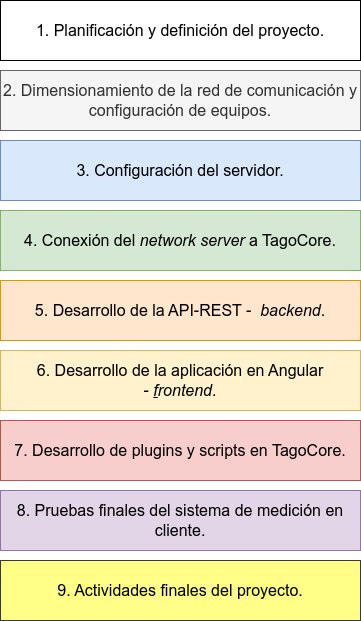
\includegraphics[width=.5\textwidth]{./Figuras/AoN_task_color.png}
\caption{ Colores del diagrama de \textit{Activity on Node}.}
\label{fig:AoN_task_color}
\end{figure}

En la figura \ref{fig:AoN} se muestra el diagrama de \textit{Activity on Node}.
\begin{figure}[htpb]
\centering 
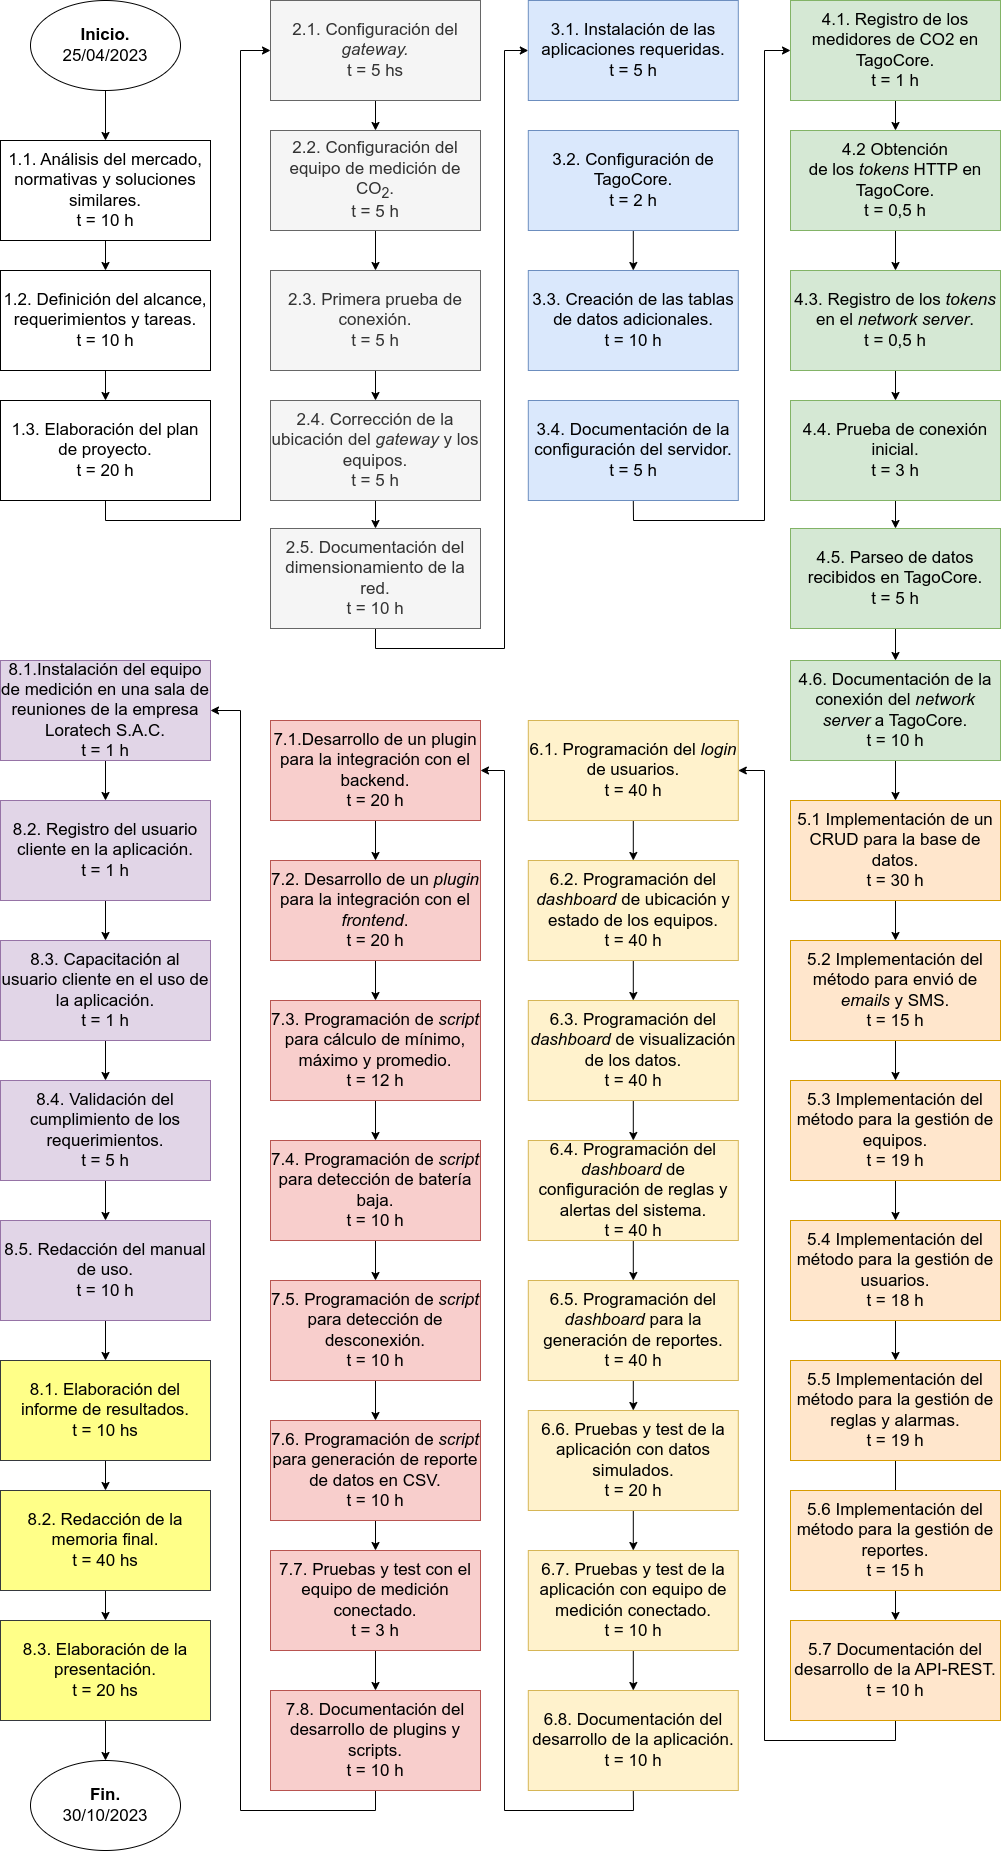
\includegraphics[width=.81\textwidth]{./Figuras/AoN.png}
\caption{Diagrama de \textit{Activity on Node}.}
\label{fig:AoN}
\end{figure}


\newpage
Todas las tareas se realizarán de forma secuencial debido a la existencia de un único recurso humano. Por lo tanto, existe un único camino que se considerá como el camino crítico.
\section{11. Diagrama de Gantt}
\label{sec:gantt}
En las figuras \ref{fig:WBS1} y \ref{fig:WBS2} se muestra la tabla con el desglose de actividades y fechas de inicio y fin.

\begin{figure}[htpb]
\centering 
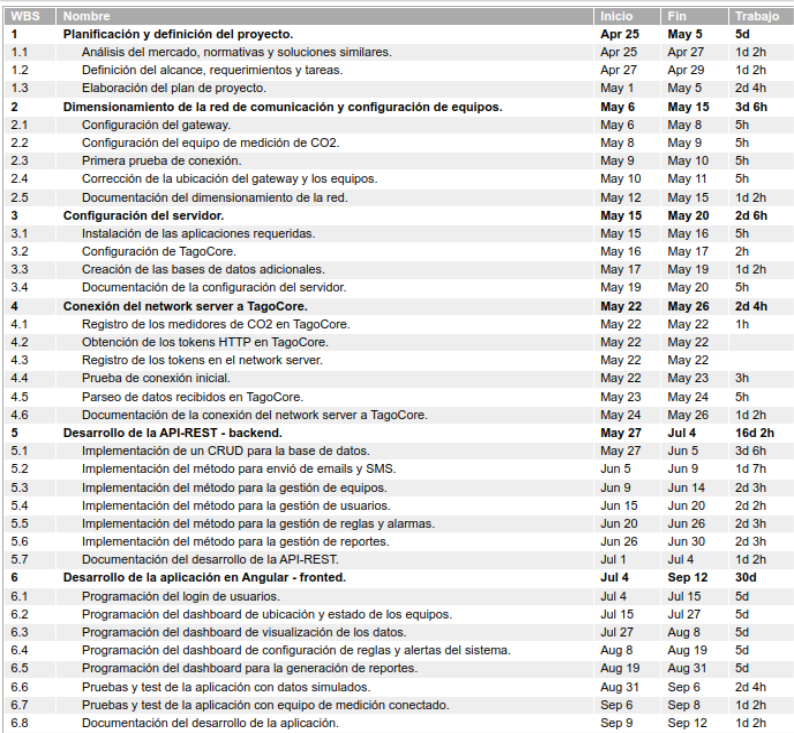
\includegraphics[width=1.0\textwidth]{./Figuras/WBS1.png}
\caption{Planificación de tareas, parte 1.}
\label{fig:WBS1}
\end{figure}

\begin{figure}[htpb]
\centering 
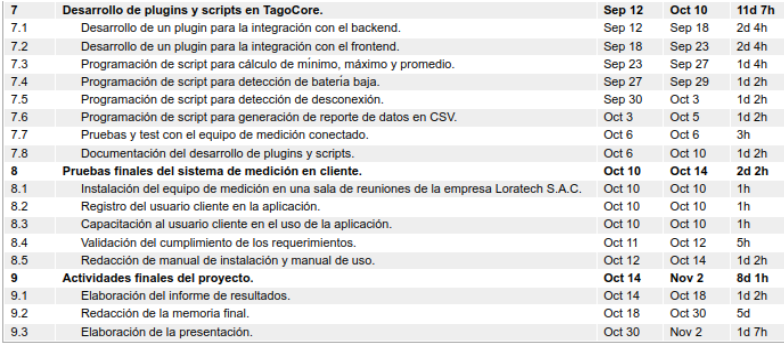
\includegraphics[width=1.0\textwidth]{./Figuras/WBS2.png}
\caption{Planificación de tareas, parte 2.}
\label{fig:WBS2}
\end{figure}

\newpage
En las figuras \ref{fig:diagGantt1}, \ref{fig:diagGantt2}, \ref{fig:diagGantt3}, \ref{fig:diagGantt4}, \ref{fig:diagGantt5} y \ref{fig:diagGantt6} se muestra el diagrama de Gantt. Para la elaboración se consideró una jornada laboral de lunes a sábado con 4 horas de trabajo diario en la empresa Loratech SAC.

\begin{figure}[htpb]
\centering 
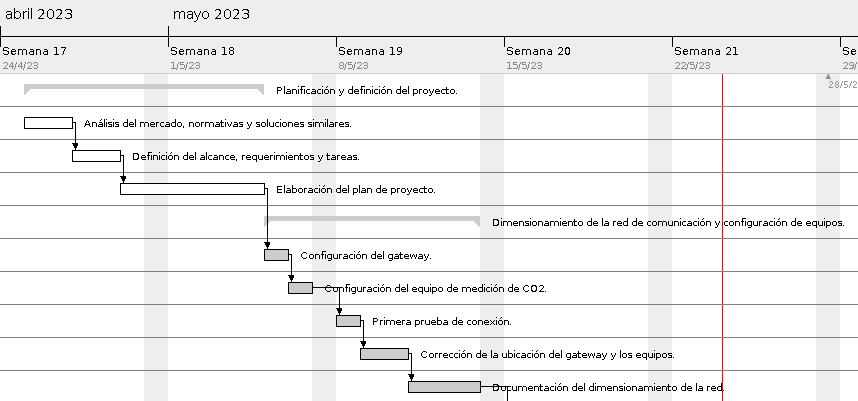
\includegraphics[height=.3\textheight]{./Figuras/Gantt1.png}
\caption{Diagrama de Gantt, parte 1.}
\label{fig:diagGantt1}
\end{figure}

\begin{figure}[htpb]
\centering 
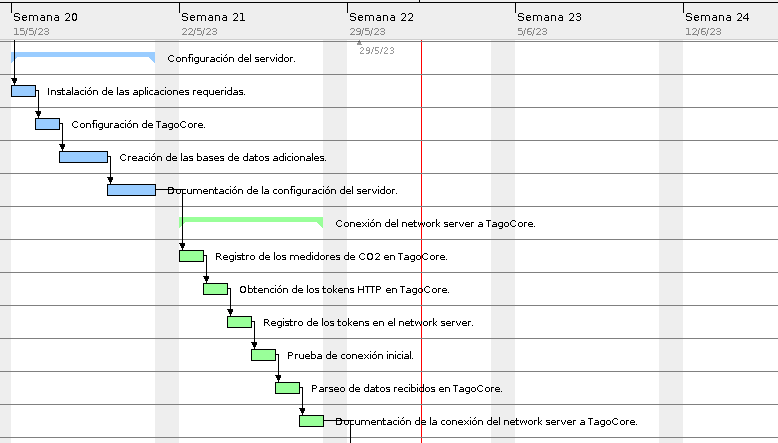
\includegraphics[height=.37\textheight]{./Figuras/Gantt2.png}
\caption{Diagrama de Gantt, parte 2.}
\label{fig:diagGantt2}
\end{figure}

\begin{figure}[htpb]
\centering 
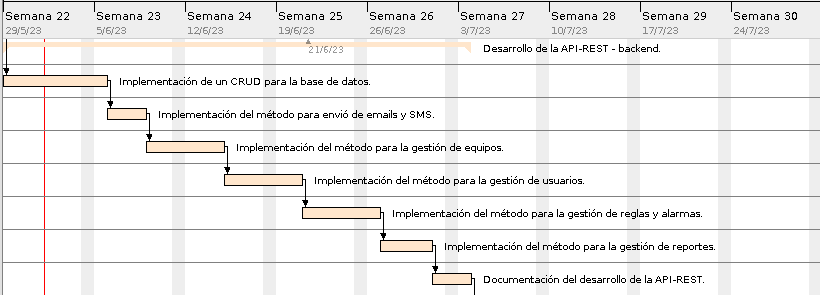
\includegraphics[height=.23\textheight]{./Figuras/Gantt3.png}
\caption{Diagrama de Gantt, parte 3.}
\label{fig:diagGantt3}
\end{figure}

\begin{figure}[htpb]
\centering 
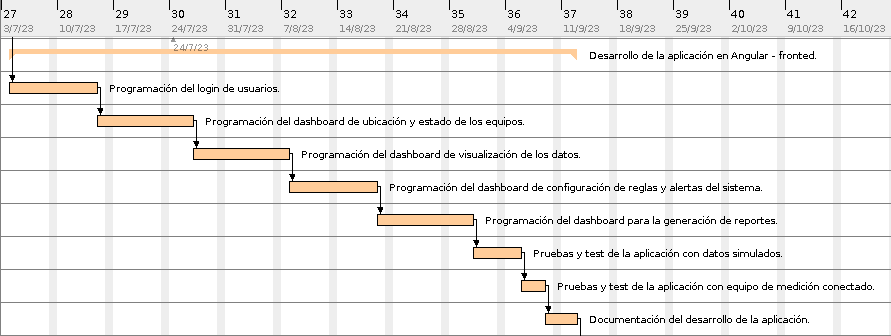
\includegraphics[height=.25\textheight]{./Figuras/Gantt4.png}
\caption{Diagrama de Gantt, parte 4.}
\label{fig:diagGantt4}
\end{figure}

\begin{figure}[htpb]
\centering 
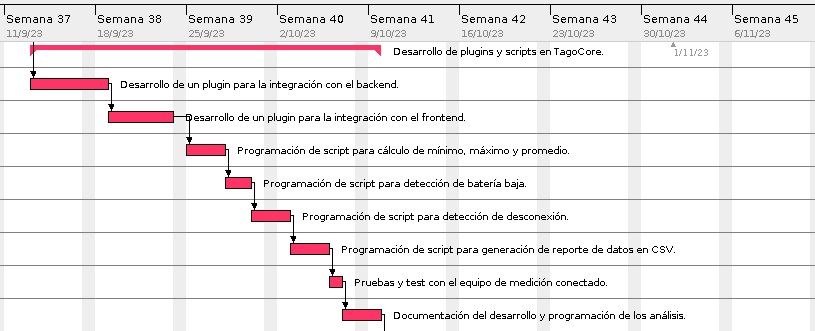
\includegraphics[height=.26\textheight]{./Figuras/Gantt5.png}
\caption{Diagrama de Gantt, parte 5.}
\label{fig:diagGantt5}
\end{figure}

\begin{figure}[htpb]
\centering 
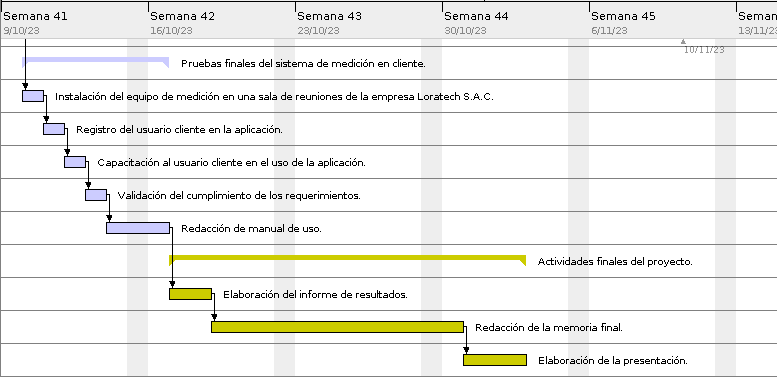
\includegraphics[height=.31\textheight]{./Figuras/Gantt6.png}
\caption{Diagrama de Gantt, parte 6.}
\label{fig:diagGantt6}
\end{figure}

\section{12. Presupuesto detallado del proyecto}
\label{sec:presupuesto}
El proyecto se ejecutará en la República del Perú. Todos los precios indicados están expresados en soles peruanos - PEN (S/. ). Al Final de cada sección se indica el precio aproximado en dólares americanos - USD. Para el tipo de cambio se consideró el valor 1 USD = 3,70 PEN. Este fue el tipo de cambio promedio del mes de mayo del año 2023.

En la siguiente tabla se presenta el presupuesto para este proyecto. 
\begin{table}[htpb]
\centering
\begin{tabularx}{\linewidth}{@{}|X|c|r|r|@{}}
\hline
\rowcolor[HTML]{C0C0C0} 
\multicolumn{4}{|c|}{\cellcolor[HTML]{C0C0C0}COSTOS DIRECTOS} \\ \hline
\rowcolor[HTML]{C0C0C0} 
\multicolumn{1}{c|}{\cellcolor[HTML]{C0C0C0}Descripción}&
\multicolumn{1}{c|}{\cellcolor[HTML]{C0C0C0}Cantidad} &
\multicolumn{1}{c|}{\cellcolor[HTML]{C0C0C0}Valor unitario} &
\multicolumn{1}{c|}{\cellcolor[HTML]{C0C0C0}Valor total} \\ \hline
Horas de ingeniería.&
\multicolumn{1}{c|}{660 h} &
\multicolumn{1}{c|}{S/30,00} &
\multicolumn{1}{c|}{S/19800,00} \\ \hline
\multicolumn{1}{|l|}{Ordenador de escritorio (servidor).} &
\multicolumn{1}{c|}{1 uni.} &
\multicolumn{1}{c|}{S/5000,00} &
\multicolumn{1}{c|}{S/5000,00} \\ \hline
\multicolumn{1}{|l|}{Uso del laboratorio de la empresa Loratech S.A.C} &
\multicolumn{1}{c|}{660 h.} &
\multicolumn{1}{c|}{S/50,00} &
\multicolumn{1}{c|}{S/33000,00} \\ \hline
\multicolumn{3}{|c|}{SUBTOTAL EN PEN} &
  	\multicolumn{1}{c|}{S/57800,00} \\ \hline
\multicolumn{3}{|c|}{SUBTOTAL EN USD} &
  	\multicolumn{1}{c|}{\$15621,62} \\ \hline  	
\rowcolor[HTML]{C0C0C0} 
\multicolumn{4}{|c|}{\cellcolor[HTML]{C0C0C0}COSTOS INDIRECTOS} \\ \hline
\rowcolor[HTML]{C0C0C0} 
\multicolumn{1}{c|}{\cellcolor[HTML]{C0C0C0}Descripción}&
\multicolumn{1}{c|}{\cellcolor[HTML]{C0C0C0}Cantidad} &
\multicolumn{1}{c|}{\cellcolor[HTML]{C0C0C0}Valor unitario} &
\multicolumn{1}{c|}{\cellcolor[HTML]{C0C0C0}Valor total} \\ \hline
\multicolumn{1}{|l|}{Se estima 30\% de los costos directos} &
\multicolumn{1}{c|}{-} &
\multicolumn{1}{c|}{S/17340,00} &
\multicolumn{1}{c|}{S/17340,00} \\ \hline
\multicolumn{3}{|c|}{SUBTOTAL EN PEN} &
  \multicolumn{1}{c|}{S/17340.00} \\ \hline
\multicolumn{3}{|c|}{SUBTOTAL EN USD} &
  \multicolumn{1}{c|}{\$4686.49} \\ \hline  
\rowcolor[HTML]{C0C0C0}
\multicolumn{3}{|c|}{TOTAL EN PEN} & 
  \multicolumn{1}{c|}{S/75140,00}\\ \hline
\rowcolor[HTML]{C0C0C0}
\multicolumn{3}{|c|}{TOTAL EN USD} &  
  \multicolumn{1}{c|}{\$20308,11}\\ \hline
\end{tabularx}%
\end{table} \newline
\section{13. Gestión de riesgos}
\label{sec:riesgos}
a) Identificación de los riesgos y estimación de sus consecuencias:

Riesgo 1: Deterioro o daño completo de alguno de los equipos del proyecto.
\begin{itemize}
	\item Severidad (S): 9.\\
	 El equipo de medición de CO$_{2}$ y el \textit{Gateway} de comunicación LoRaWAN son fundamentales para el proyecto. El daño o deterioro implicaría hacer una compra no contemplada, esto ocasionaría de retrasos en el cronograma y un gasto mayor de recursos.
	\item Probabilidad de ocurrencia (O): 3 .\\
	En el dimensionamiento de la red de comunicación y configuración de equipos, debido a la manipulación de los equipos, puede ocurrir algún tipo de deterioro o daño no previsto. 
\end{itemize}  

Riesgo 2: Deterioro o daño del ordenador de escritorio que se usará como servidor.
\begin{itemize}
	\item Severidad (S): 10.\\
	 El servidor es la parte más importante de nuestro proyecto, ya que la mayor cantidad de horas de desarrollo se realizará sobre él. Un deterioro o daño en el equipo ocasionaría la paralización temporal del proyecto hasta su reposición, debido a que el equipo es parte de los activos de la empresa. 
	\item Probabilidad de ocurrencia (O): 1 .\\
	La empresa cuenta con un ambiente adecuado y respaldo de energía para el funcionamiento del ordenador. Se destinará el uso de este equipo a exclusividad del proyecto, de esta manera las probabilidades de daño por manipulación de un tercero serán mínimas.
\end{itemize} 

Riesgo 3: Nueva reglamentación que disponga el Ministerio de Salud y Ministerio de Trabajo, que incluya características adicionales al sistema de medición de CO$_{2}$ no contemplados.
\begin{itemize}
	\item Severidad (S): 10.\\
	 La motivación principal del proyecto es atender la nueva demanda de equipos de medición de CO$_{2}$  que están teniendo las empresas. Cambios en el reglamento y características técnicas podrían paralizar el proyecto temporalmente hasta que se pueda validar si es necesario un replanteamiento o podremos seguir con lo desarrollado.
	\item Probabilidad de ocurrencia (O): 7.\\
	El escenario político actual en la República del Perú hace que existan altas probabilidades de cambios de las autoridades que laboran en los ministerios, esto puede traer como consecuencia modificaciones a las normas de seguridad laboral ya existentes.
\end{itemize} 

Riesgo 4: Conflictos sociales que impidan el trabajo presencial en el laboratorio de la empresa.
\begin{itemize}
	\item Severidad (S): 5.\\
	 Hay varias zonas del país donde todavía se llevan a cabo protestas con motivos políticos. Dado que la ubicación de la empresa se encuentra en una zona propensa a actos de vandalismo durante las protestas, siempre se suspenden las labores presenciales durante los días de protesta. Esto se hace con el objetivo de proteger la integridad y seguridad de los trabajadores. Durante estos días no se podrá avanzar con las actividades previstas.
	\item Probabilidad de ocurrencia (O): 3.\\
	Aún es posible que se produzcan protestas en la ciudad de Lima, aunque con el paso de los meses la probabilidad de que ocurran irá disminuyendo. 
\end{itemize} 


Riesgo 5: Retraso debido a imprevistos laborales con la empresa.
\begin{itemize}
	\item Severidad (S): 9.\\
	La empresa tiene otros proyectos que pueden requerir realizar viajes fuera de la ciudad. Durante los viajes será imposible avanzar con el proyecto lo que podría generar retrasos.
	\item Probabilidad de ocurrencia (O): 5.\\
	Se coordino con la empresa para reducir al mínimo la programación de viajes en el presente año, con el objetivo de poder avanzar el proyecto. Sin embargo, existe la posibilidad de que ocurra.
\end{itemize} 
 

b) Tabla de gestión de riesgos:

\begin{table}[htpb]
\centering
\begin{tabularx}{\linewidth}{@{}|X|c|c|c|c|c|c|@{}}
\hline
\rowcolor[HTML]{C0C0C0} 
Riesgo & S & O & RPN & S* & O* & RPN* \\ \hline
Deterioro o daño completo de alguno de los equipos del proyecto.&9&3&\textcolor{red}{27}&9&1&9      \\ \hline
Deterioro o daño del ordenador de escritorio que se usará como servidor.&10&1&10&-&-&-     \\ \hline
Nueva reglamentación que disponga el Ministerio de Salud y Ministerio de Trabajo, que incluya características adicionales al sistema de medición de CO$_{2}$ no contemplados.&10&7&\textcolor{red}{70}&2&7&14    \\ \hline
Conflictos sociales que impidan el trabajo presencial en el laboratorio de la empresa.&5&3&15&-&-&-    \\ \hline
Retraso debido a imprevistos laborales con la empresa.&9&5&\textcolor{red}{45}&5&2&10     \\ \hline
\end{tabularx}%
\end{table}

Criterio adoptado: 
Se tomarán medidas de mitigación en los riesgos cuyos números de RPN sean mayores o iguales a 25.

Nota: los valores marcados con (*) en la tabla corresponden luego de haber aplicado la mitigación.\\


c) Plan de mitigación de los riesgos que originalmente excedían el RPN máximo establecido:
Se trabajará en un plan de mitigación para los riesgos 1, 5, 6 y 7, ya que exceden el valor máximo admitido: 25.

Riesgo 1: Se acondicionará un almacén temporal para lo equipos del proyecto, una mesa de trabajo exclusivo en el laboratorio y  en un área reservado solo para el proyecto. Ademas se adquirirá  algunos equipos de \textit{backup}.
\begin{itemize}
  \item Severidad (S): 9. \\
  La severidad se mantiene.
  \item Probabilidad de ocurrencia (O): 1.\\
  Con las medidas adoptadas, es muy poco probable que se deterioren o dañen los equipos. Ademas, al contar con un área reservada para el proyecto, se evita que personal ajeno pueda manipular los equipos. Finalmente los \textit{backup} de equipos permitirán continuar con el proyecto en caso algo de lo anterior falle.
\end{itemize}

Riesgo 3: Se conversará con el cliente sobre esta posibilidad y se llegará a un acuerdo, previo análisis de los cambios. Si los cambios no son complejos y si se ajustan dentro de los plazos establecidos, se harán las modificaciones en el plan de proyecto. Caso contrario, se considerarán para una segunda etapa después de finalizar este proyecto.
\begin{itemize}
  \item Severidad (S): 2. \\
  Se reduce la severidad, por que se acordó que se mantendría el plan proyecto, y solo si el cambio no implica modificar significativamente la planificación se podría tomar en cuenta.
  \item Probabilidad de ocurrencia (O): 7.\\
  La probabilidad se mantiene, ya que es un evento externo a la empresa.
\end{itemize}

Riesgo 5: Se conversará con el cliente pará buscar compañero de reemplazo para los viajes. Solo en casos excepcionales se podrá paralizar temporalmente la ejecución del proyecto, pero luego se recuperará durante la jornada laboral, dedicando tiempo completo según acuerdo. La empresa se compromete a usar esto como ultimo recurso ya que la finalización de este proyecto esta dentro de sus intereses comerciales.
\begin{itemize}
  \item Severidad (S): 5. \\
   La severidad se reduce, ya que habrá posibilidad de dedicar más tiempo dentro de la jornada laboral en caso se retrase el proyecto.
  \item Probabilidad de ocurrencia (O): 2.\\
  La probabilidad se reduce, ya que hay un compromiso de la empresa por evitar en lo posible este escenario.
\end{itemize}


\section{14. Gestión de la calidad}
\label{sec:calidad}
Se presenta a continuación los requerimientos con sus verificaciones y validaciones.

\begin{enumerate}
	\item Req 1,3: La red de comunicación deberá tener la capacidad de brindar cobertura total en los ambientes laborales. Se establece como requisito que los valores de RSSI (indicador de la fuerza de la señal recibida) en los equipos de medición sean superiores a -120 dBm.
	\begin{itemize}
		\item Verificación: Se verificará en los equipos, en el \textit{network server} y con un \textit{tester} LoRaWAN que los niveles de RSSI sean mayores a -120 dBm.
		\item Validación: no aplica.
	\end{itemize}
	\item Req 1.1, 1.2, 1.4, 1.5, 1.6 y 1.7: Requerimientos de los equipos.
	\begin{itemize}
		\item Verificación: Se revisará los manuales, hojas de datos e información de soporte por parte del fabricante, para verificar que se cumpla el protocolo de comunicación, los rangos de frecuencia de operación y las especificaciones técnicas de los equipos.
		\item Validación: no aplica.
	\end{itemize}
	\item Req 2.1, 2.2, 2.3, 2.4 y 2.5: Requerimientos del sistema de gestión y monitoreo de medidores de CO${_2}$ (\textit{backend}).
	\begin{itemize}
		\item Verificación: Se revisará la version del sistema y cada una de las aplicaciones instaladas en el servidor. Se revisara los códigos para verificar el uso de cada programa instalado.
		\item Validación: no aplica.
	\end{itemize}
	\item Req 2.6, 2.7 y 2.8: Requerimientos del sistema de gestión y monitoreo de medidores de CO${_2}$ (\textit{frontend}).
	\begin{itemize}
		\item Verificación: Se revisará el código de implementación, se iniciará sesión en la aplicación web y se revisará la consola del navegador. Se verificará cada \textit{dashboard} y la información presentada.
		\item Validación: Se registrará al cliente en la aplicación. El cliente validará la visualización de los datos en la aplicación y configurará los valores para las alertas.
	\end{itemize}
	\item Req 3.1, 3.2, 3.3 y 3.4: Requerimientos de documentación.
	\begin{itemize}
		\item Verificación: Se revisara la entrega de la documentacion y manuales generados. Asimismo se verificará la carga exitosa de los codigos desarrollados en el repositorio GitHub de la compañía.
		\item Validación: El cliente dará su conformidad por cada documento generado, así como por el código subido al repositorio de GitHub.
	\end{itemize}
	\item Req 4.1 y 4.2: Requerimiento de \textit{testing}
	\begin{itemize}
		\item Verificación: Se generará datos simulados desde \textit{network server} para probar cada funcionalidad de la aplicación. Se verificara la base de datos y las alarmas generadas.
		\item Validación: El cliente realizará la configuración del sistema, validando la funcionalidad con la generación de las alarmas, notificaciones y generación de reportes.
	\end{itemize}
\end{enumerate}

\section{15. Procesos de cierre}    
\label{sec:cierre}
Las actividades del proceso de cierre estarán a cargo del responsable del proyecto \authorname.


\begin{itemize}
	\item Pautas de trabajo que se seguirán para analizar si se respetó el plan de proyecto original:
	 \begin{itemize}
	 \item[-]Una vez finalizado cada bloque de tareas, durante de la documentación, se hará una análisis del grado de cumplimento de los objetivos y requerimientos.
	 \item[-]Se analizará las horas empleadas en cada bloque de tareas, en caso que la estimación haya sido en exceso se aprovechará en avanzar las siguientes tareas. Si hubo tareas que no se estimaron correctamente, se tratará de reorganizar las actividades con tal de no afectar la fecha de entrega final.
	 \item[-]Se tomará nota de aquellas tareas que pudieron haberse hecho en paralelo y aquellas cuyo alcance inicial estaba sobredimensionado para el proyecto.
	 \end{itemize} 
	\item Identificación de las técnicas y procedimientos útiles e inútiles que se emplearon, y los problemas que surgieron y cómo se solucionaron:
	\begin{itemize}
	 \item[-]Se incluirá en la documentación entregable del proyecto aquellos aciertos y desaciertos durante la ejecución del proyecto. Las técnicas más útiles y aquellos procesos que pudieron afrontarse de mejor manera también serán incluidos como comentarios.
	 \item[-]En el informe final del proyecto se analizarán las oportunidades de mejora. Estas podrán se tomadas en consideración en la planeación de futuros proyectos.
	 \item[-] Se analizará aquellas tareas que fueron más complicadas y los riesgos que se materializaron, a fin de documentar si las acciones de mitigación tuvieron el efecto esperado.
	 \end{itemize} 
	\item Acto de agradecimiento a todos los interesados, al equipo de trabajo y colaboradores:
	\begin{itemize}
	\item[-]En la memoria técnica se incluirá un apartado para los agradecimiento a todos los que colaboraron con el desarrollo del proyecto.
	\item[-]Previo a la presentación ante el jurado, se tendrá una presentación de resultados a la empresa, que estará precedida por el cliente y auspiciador del proyecto. Se indicarán los objetivos alcanzados, proyectos a futuro y se darán los agradecimientos correspondientes.
	\item[-]Después de la presentación y sustentación ante el jurado, se realizará un agradecimiento público al director, jurado, revisores y docentes que colaboraron con el proyecto. 
	 \end{itemize}
\end{itemize}

\end{document}
